% !TEX root = ../../../main.tex
% 来源：中学数学实验教材·第三册（高中数学）
% 章节：函数及其图象 / 函数及其图象
% 原始文件：4.tex，行 492-507
% 类型：tikz
% ---
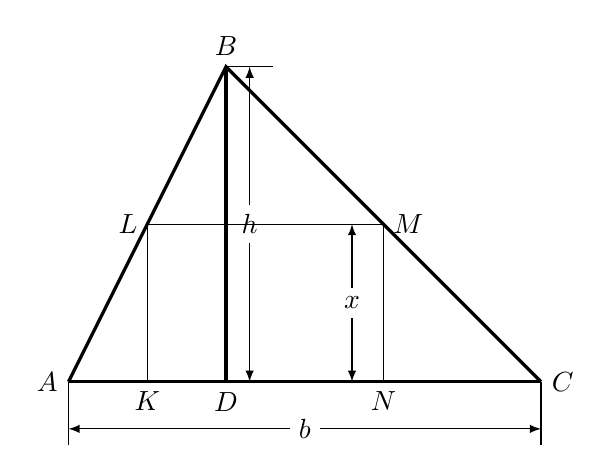
\begin{tikzpicture}[>=latex]
\draw[very thick] (0,0)node[left]{$A$}--(6,0)node[right]{$C$};
\draw[very thick] (0,0)--(2,4)node[above]{$B$}--(6,0);
\draw[very thick] (2,4)--(2,0)node[below]{$D$};  
\draw[<->](2.3,0)--node[fill=white]{$h$}(2.3,4);
\draw (1,0)node[below]{$K$}--(1,2)node[left]{$L$} --(4,2)node[right]{$M$}-- (4,0)node[below]{$N$};
\draw (2,4)--(2.6,4);

\draw[<->](3.6,0)--node[fill=white]{$x$}(3.6,2);
\foreach \x in {0,6}
{
    \draw (\x,0)--(\x,-.8);
}
\draw[<->](0,-.6)--node[fill=white]{$b$}(6,-.6);

\end{tikzpicture}
